\documentclass[12pt,a4paper]{report}

\usepackage[utf8]{inputenc}
\usepackage[russian]{babel}
\usepackage[T2A]{fontenc}
\usepackage{indentfirst}
\usepackage{listings}
\usepackage[normalem]{ulem}
\usepackage{ccaption}\captiondelim{. }
\usepackage{remreset}
\usepackage{graphicx}\graphicspath{{pictures/}}
\usepackage{array}
\usepackage{hyphenat}


\usepackage{xcolor}
\renewcommand{\ULthickness}{1pt}
\newcommand\bad{\bgroup\markoverwith{\textcolor{red}{\rule[.5ex]{5pt}{1pt}}}\ULon}
\newcommand\rmk[1]{\textcolor{red}{#1}}

\usepackage[margin=2cm,left=3cm,includefoot]{geometry}
\renewcommand{\baselinestretch}{1.5}
\parindent=1.25cm
\newcommand{\chapters}[1]{\chapter*{#1}\addcontentsline{toc}{chapter}{#1}}
\def\labelitemi{---}
\def\labelitemii{---}
\lstset{columns=fullflexible,extendedchars=true,showstringspaces=false}

% Добавление подсветки для diff листингов
\lstdefinelanguage{diff}
{
keywords={+, -, \ , @@, diff},
sensitive=false,
morecomment=[l][""]{\ },
morecomment=[l][\emph]{+},
morecomment=[l][""]{-},
morecomment=[l][\textbf]{@@},
morecomment=[l][""]{diff}
}

\frenchspacing
\clubpenalty=10000
\widowpenalty=10000
\frenchspacing

% TODO: Appendix head style
% TODO: Table layout
% TODO: Содержание, Список использованных источников

\makeatletter
% Chapter heads
\def\@makechapterhead#1{%
  \vspace*{0\p@}%
  {\parindent \z@ \raggedright \normalfont
    \interlinepenalty\@M
    \huge \bfseries%
    \ifnum \c@secnumdepth >\m@ne
        \huge\bfseries \thechapter \quad
    \fi%
    #1\par\nobreak
    \vskip 20\p@
  }}
\def\@makeschapterhead#1{%
  \vspace*{0\p@}%
  {\parindent \z@ \raggedright
    \normalfont
    \interlinepenalty\@M
    \Huge \bfseries  #1\par\nobreak
    \vskip 20\p@
  }}
% Points in reference labels
\renewcommand{\@biblabel}[1]{#1.\hfill}
% Figure enumeration
\@removefromreset{figure}{chapter}
\renewcommand{\thefigure}{\@arabic\c@figure}
\makeatother

\newcommand{\inspicture}[3]{
\begin{figure}[hb!]
\centering
\includegraphics[width=#3\textwidth]{#1.pdf}
\caption{#2}
\label{picture:#1}
\end{figure}
}

\begin{document} 
\thispagestyle{empty}

\enlargethispage{2cm}
{
\renewcommand{\baselinestretch}{1.25}
\selectfont

\begin{center}
МИНОБРНАУКИ РОССИИ

Федеральное государственное бюджетное образовательное\\ учреждение
высшего профессионального образования\\
«Ярославский государственный университет им.~П.\,Г. Демидова»

Кафедра компьютерных сетей

\vspace{1.5cm}

\hfill\parbox{6.5cm}
{ 
<<Допустить к защите>>

Заведующий кафедрой

д.\,ф.-м.\,н., профессор \\
\hbox to 2cm{\hrulefill} С.\,Д.~Глызин

<<\hbox to 0.5cm{\hrulefill}>> \hbox to 2.3cm{\hrulefill} 2012 г.
}

\vspace{2.5cm}

{\bf \em Дипломная работа}
\par по специальности 010501.65 Прикладная математика и информатика

% {\bf \em Выпускная квалификационная работа бакалавра}
% \par по направлению 010500.62 Прикладная математика и информатика

% {\bf \em Магистерская диссертация}
% \par по направлению 010500.68 Прикладная математика и информатика

\vspace{0.5cm}

{ \large \bf \selectfont Название работы
  
}

\vspace{3cm}


\hfill\parbox{6.5cm}
{ 
Научный руководитель

ст. преподаватель\\
\hbox to 1.5cm{\hrulefill} И.\,В.~Парамонов

<<\hbox to 0.5cm{\hrulefill}>> \hbox to 2.3cm{\hrulefill} 2012 г.
}

\vspace{1.5cm}

\hfill\parbox{6.5cm}
{ 
Студент группы ИВТ-52СО\\
\hbox to 1.5cm{\hrulefill}

<<\hbox to 0.5cm{\hrulefill}>> \hbox to 2.3cm{\hrulefill} 2012 г.
}

\vspace{4cm}

Ярославль 2012
 
\end{center}
}

\newpage

%%% Local Variables: 
%%% mode: latex
%%% TeX-PDF-mode: t
%%% TeX-master: "diploma"
%%% End: 

\tableofcontents
\newpage

\chapter*{Введение}
\label{chap:introduction}
\addcontentsline{toc}{chapter}{Введение}

В настоящее почти каждый человек, живущий в развитой стране, использует
мобильные устройства в своём быту. Существует множество классов данных
устройств, таких как: мобильные телефоны, смартфоны, КПК, планшеты. Мобильные
устройства прочно вошли в жизнь человека. С каждым годом наращивается функционал
и производительность данных устройств. Многие люди находят в данных устройствах
замену своему стационарному компьютеру. Мобильные устройства оснащаются
средствами связи, такими как wi-fi, bluetooth, 3G, что позволяет обладателю
данного устройства пользоваться интернетом.

Диаграммы связей --- это графическое представление данных, имеющих
иерархическую структуру. Они позволяют создавать, отображать и
структурировать некоторую иноформацию. У диаграмм связи нет ограничений на
структуру данных, за исключением иерархческого порядка, поэтому они могут
использоваться для работы с различной инофрмацией. Они успешно
применяются для генерации идей, конспектирования докладов, написания планов
статей, составление презентаций и так далее.

Диаграммы связи используются во множестве различных ситуаций связанных с работой
над данными. Зачастую работа над данными требует участия группы людей. В данной
ситуации возникает несколько проблем. Во-первых, людям, участвующим в данном
процессе необходимо собраться в одном месте, чтобы начать совместную работу.
Во-вторых, сложно предоставить всем участникам процесса равноценный доступ к
диаграмме связи, например только один человек может сидеть за компьютером, либо
писать на доске.

Решение вышеназванных проблем заключается в том, чтобы использовать возможности
мобильных устройств. Мобильные устройства портативны, что позволяет их с
легкостью всегда держать при себе. Также они оснащены средствами доступа в
интернет. Идея заключается в том, чтобы предоставить людям равные возможности по
внесению своего вклада в создание диаграмм, в любое время, в любом месте,
используя мобильное устройство или персональный компьютер.

В данной работе описывается реализация функции совместного редактирования в
редакторе диаграмм связей под названием HiveMind. Данный проект разрабатывается
с начала 2010 года группой студентов рамках программы FRUCT. HiveMind имеет
множество функций для редактирования диаграмм связей и поддержку платформ
Windows, Maemo, MeeGo, Linux. Проект направлен на достижение максимальной
мобильности пользователей, повышение производительности труда и увеличение
потенциальных решений в поставленных задачах.


\chapter{Общая характеристика предметной области и постановка задачи}
\section{Системы управления проектом}
\subsection{Назначение систем управления проектом}

Системы управление проектами являются комплексными системами, которые
предоставляют большой спектр функциональных возможностей для деятельностей,
связанных с разработкой проектов. Функционал, обеспечивающий следующие виды
деятельности, присутствует во многих системах управления проектами:
\begin{itemize}
  \item планирование;
  \item постановка задач;
  \item оценка и разработка;
  \item управление бюджетом;
  \item распределение ресурсов;
  \item контроль качества;
  \item взаимодействие;
  \item документирование.
\end{itemize}
Системы управления проектами позволяют сделать процесс разработки более
эффективным и удобным, таким образом уменьшая сложность ведения проекта и
позволяя осуществлять управление большим количеством проектов. 

Одна из основных возможностей систем управления проектами "--- это
управление множеством событий и задач. Основные действия, производимые
при управлении задачами, следующие:
\begin{itemize}
  \item разрешение зависимостей между задачами;
  \item назначение задач участникам проекта;
  \item решение проблем, связанных с неточной оценкой срока выполнения задач.
\end{itemize}

При помощи систем управления проектами возможно выполнять множество задач
связанных с планированием, поскольку они предоставляют участникам проекта
информацию, необходимую для измерения текущих затрат на проект, и помогают
оценить объем работ и сроки, необходимые для завершения проекта. Следующая
информация может быть предоставлена системой управления проектами:
\begin{itemize}
  \item ожидаемое время выполнения задач;
  \item предупреждения о возможных рисках в проекте;
  \item объём выполняемых работ;
  \item прогресс проекта (настоящие и ожидаемые результаты);
  \item стоимость разработки.
\end{itemize}

\subsection{Соответствие функционала запросам организации}
Ярославская лаборатория FRUCT \cite{yarfruct} разрабатывает мобильные
приложения для различных платформ, таких как: MeeGo, Symbian, Android. На
текущий момент ведётся разработка более 5 проектов, участниками которых
являются студенты факультета ИВТ.

Мир информационных технологий чрезвычайно быстро развивается и изменяется.
Таким образом менеджеры и участники проектов постоянно сталкиваются с
изменением требований и оперируют большим количеством информации. Управление
проектами в информационных областях является сложным процессом, облегчить
выполнение которого могут системы управления проектами.

Система управления проектами должна быть легко расширяемой, для того чтобы
удовлетворять новым требованиям. Миграция на другую систему управления
проектами в большинстве случаев невозможно из-за различия структур данных в БД
и сложных взаимосвязей между внутри БД. По этой причине одним из важных
требований к системам управления проектами в информационных областях является
возможность расширения.

\section{Система управления проектами Redmine}
Redmine \cite{redmine} "--- это система управления проектами, основными
достоинствами которой являются, бесплатность, гибкая расширяемость, доступные
исходные коды. Данная система позволяет управлять всеми стадиями разработки
проекта, начиная от обсуждения проектного плана и заканчивая отслеживанием
задач и занесением данных об их прогрессе в общую базу знаний проекта. Одной из
главных особенностей Redmine является большое сообщество разработчиков,
сложившееся вокруг него. Redmine "--- это Open Source проект и каждый желающий
может принять участие в его разработке, тем самым способствуя развитию проекта.

\subsection{Функциональные возможности}
Redmine обладает следующими возможностями:
\begin{itemize}
  \item неограниченное количество проектов;
  \item гибкая система контроля доступа;
  \item гибкая система отслеживания задач;
  \item диаграмма Ганта и календарь;
  \item новости, документы и управление файлами;
  \item RSS и уведомления по e-mail;
  \item вики-страницы;
  \item форумы;
  \item отслеживание времени;
  \item настраиваемые поля для задач, проектов и пользователей;
  \item интеграция с системами контроля версий;
  \item создание задач посредством e-mail;
  \item аутентификация через LDAP;
  \item регистрация инициируемая пользователем;
  \item поддержка множества языков;
  \item поддержка нескольких БД.
\end{itemize}
Проект активно развивается и с выходом новых версии добавляются новые
возможности.

\section{Ruby on Rails}
Redmine разработан с помощью фреймворка Ruby on Rails \cite{rails}. Ruby on
Rails "--- это фреймворк, написанный на языке Ruby \cite{ruby}, предназначенный
для построения веб-приложений в соответствии с шаблоном проектирования
Модель-Вид-Контроллер. Rails приложение состоит из трёх ключевых уровней,
описанных ниже.

Уровень представления состоит из файлов-шаблонов, которые отвечают за
отображение данных приложения. Шаблоны могут быть различных видов, но основным
форматом является HTML со вставками на языке Ruby, за генерацию которого
отвечает движок ERB языка Ruby.

Уровень модели представляет доменную область и инкапсулирует бизнес-логику
приложения. Классы модели в Rails приложении могут быть связаны с базой данных
(БД) через Rails модуль ActiveRecord. ActiveRecord даёт возможность работать со
строками в БД как с объектами, а также дополнять данные объекты методами
бизнес-логики.

Контроллеры отвечают за обработку входящих HTTP запросов и формирование ответа.
Зачастую, ответ возвращается в HTML, но также возможна генерация ответа в XML,
JSON, PDF и других форматах. Контроллеры генерируют ответ на основе данных,
полученных из моделей, и соответствующих шаблонов представления.

\subsection{Возможности для расширения}
Существует два способа расширить функциональность Redmine: непосредственное
изменение исходного кода и оформление изменений в виде патчей или разработка 
модулей к системе, которые называются плагинами.

\subsubsection{Патч}
Изменение функциональности с помощью патча является универсальным способом,
применимым к любому приложению с открытыми исходными кодами. Патч представляет
собой файл, в котором отражены различия между двумя версиями исходных кодов
приложения. Пользователи или разработчики должны установить патч, для того
чтобы внести изменения в приложение. Процесс установки может быть осуществлён
вручную или автоматически, при помощи специальных утилит, таких как ``patch" в
UNIX системах. Механизм патчей позволяет удобным образом распространять
изменения исходного кода приложения.

\subsubsection{Плагин}
Плагин "--- это модуль, который подключается к приложению, с целью изменения
или добавления функциональности. Приложение предоставляет механизмы, которые
позволяют плагину зарегистрировать себя в приложении и использовать сервисы
предоставляемые приложением. Плагины зависят от сервисов предоставляемых
приложением и зачастую отдельно не используются. Приложение управляет
плагинами, предоставляя пользователям возможность динамически добавлять и
обновлять плагины без необходимости внесения изменений в основное приложение.
Система плагинов Redmine основана на механизме фреймворка Ruby on Rails,
называемом Engines. Rails Engine позволяет встроить одно Rails приложение или
часть его функциональности в другое Rails приложение.

\subsubsection{Сравнение способов расширения}
У каждого из способов есть свои достоинства и недостатки, которые приведены в
таблице \ref{comparing_extensions}.
\begin{table}[hb!]

\makeatletter
\def\@makecaption#1#2{
  \vskip\abovecaptionskip
  \sbox\@tempboxa{#2 #1}
  \begin{flushright}
    #1
  \end{flushright}
  \begin{center}
    \textbf{#2}
  \end{center}
  \vskip\belowcaptionskip}
\makeatother

\caption{Сравнение способов расширения Redmine}
\small
\centering
\begin{tabular}{ 
|>{\centering\arraybackslash}m{0.4\textwidth}
|>{\centering\arraybackslash}m{0.25\textwidth}
|>{\centering\arraybackslash}m{0.25\textwidth}|}
\hline
\textbf{Сравниваемый параметр} & \textbf{Плагин} & \textbf{Патч}\\
\hline
Сложность разработки & Высокая & Низкая \\
\hline
Спектр решаемых задач & Ограниченный & Максимальный\\
\hline
Устойчивость к обновлениям системы & Высокая & Низкая \\
\hline
Стоимость внесения изменений & Высокая & Средняя \\
\hline
Удобство распространения & Высокое & Низкое \\
\hline
\end{tabular}

\label{comparing_extensions}
\end{table}

Плагины гораздо более сложны в разработке, поскольку необходимо использовать
механизмы предусмотренные системой плагинов и возможности языка, для того,
чтобы изменить поведение приложения. Там где при использовании патча будет
достаточным внести изменения в одну строку кода, в плагинах придётся искать
способ выполнить подобное действие с помощью возможностей, предоставляемых
системой плагинов.

С помощью плагинов возможно внести изменение только непосредственно в код
приложения и невозможно изменить внешний скрипт не управляемый приложением.
Патчи решают подобную задачу стандартным способом. Таким образом патчи гораздо
более мощный инструмент модфикации приложения.

Плагины более устойчивы обновлениям системы, поскольку изменения вносятся на
более высоком уровне, с помощью предоставляемых механизмов. Успех применения
патча будет сильно зависеть, от внутреннего устройства класса и следовательно
он будет менее устойчивым к обновлениям этого класса.

Внесение изменений как в патч так и в плагин затратная операция. Но патч в
данном случае выигрывает у плагина. Поскольку плагины сложны в разработке и не
так гибки как патчи, то может потребоваться время, чтобы внести изменения или
внедрить новую функциональность в приложение.

Удобство распространения гораздо выше у плагина. Во-первых, при установке патча
возможен конфликт с одним из уже установленных патчей. Такие конфликты в случае
плагинов менее вероятны. Во-вторых, в плагине могут быть явно указаны версии
приложения с которыми он совместим или могут быть указаны зависимости от других
плагинов. В-третьих, для установки плагина не нужно уметь использовать
инструменты для применения патчей. Всё это делает плагины удобным средством
распространения расширений.

\section{Постановка задачи}
Задача по разработке расширений состоит из трёх частей:
\begin{itemize}
  \item реализация расширений;
  \item создание инфраструктуры, упрощающей поддержку расширений;
  \item размещение расширений в открытом доступе;
\end{itemize}
   
Всё взаимодействие участников проекта проходит через Redmine и важно, чтобы
работа с Redmine была эффективной, удобной и отвечала нуждам организации.
Следующая функциональность должна быть добавлена в приложение:
\begin{itemize}
  \item ораничение доступа к репозиториям;
  \item ограничение доступа к отдельным вики-страницам;
  \item рассылка уведомлений о приближающихся и просроченных
  задачах; 
  \item выбор типа задачи при составлении обзора кода;
  \item улучшение механизма позиционирования всплывающего календаря;
  \item изображения-ссылки на рекомендуемые ресурсы в боковой панели.
\end{itemize}

Разработку расширений целесообразно производить итеративно, постепенно расширяя
функциональность и исправляя дефекты. А также необходимо осуществлять поддержку
созданных расширений, поскольку Redmine регулярно обновляется и возможно, что
одно из подобных обновлений сделает некоторые расширения неработоспособными и
они потребуют соответствующих изменений. Исходя из этого, необходимо
разработать механизм позволяющий эффективно управлять итеративной разработкой и
поддержкой большого количества расширений.

Redmine "--- это Open Source проект, который развивается разработчиками по
всему миру. В интересах лаборатории способствовать тому, чтобы популярность
Redmine росла, поскольку количество энтузиастов, участвующих в его разработке,
напрямую зависит от популярности проекта. Открыв доступ к расширениям можно
привлечь сторонних разработчиков, которые помогут развивать выложенные
расширения. Необходимо выложить в открытый доступ разработанные расширения для
того, чтобы увеличить функционал и тем самым создать конкурентные преимущества
Redmine относительно других систем управления проектами.

\subsubsection{Требования к расширениям}

\paragraph{Ограничение доступа к вики-страницам.}
\label{definition:private_wiki}
Система контроля доступа в Redmine позволяет ограничить доступ ко всем
вики-страницам в проекте, но нет возможности ограничить просмотр лишь отдельных
вики-страниц. Были определены следующие требования к расширению:
\begin{itemize}
  \item должны быть реализованы права доступа на управления закрытыми
  страницами и на их просмотр;
  \item только пользователи с соответствующими правами могут просматривать
  вики-страницы и управлять из видимостью;   
  \item на вики-странице должен присутствовать элемент управления, позволяющий
  изменить её видимость;
  \item на вики-странице должен быть индикатор, указывающий, что страница
  является закрытой.
\end{itemize}

\paragraph{Ограничение доступа к репозиториям.}
\label{definiton:private_repository}
В лаборатории система управления проектами Redmine используется не только для
внутренних целей, но также позволяет внешним пользователям следить за развитием
общедоступных проектов. Но если разрешить неавторизованным пользователям
просматривать репозитории всех проектов, то невозможно запретить доступ к
одному из репозиториев, остальные оставляя открытыми. Были сформированы
следующие требования к расширению:
\begin{itemize}
  \item должно быть реализовано право доступа на просмотр закрытых
  репозиториев;
  \item закрытый репозиторий должен быть виден только пользователям с
  соответствующими правами;  
  \item вся информация, связанная с закрытым репозиторием, должна быть скрыта
  от пользователя, если у него нет соответствующих прав;
  \item на странице свойств репозитория должен присутствовать элемент
  управления, позволяющий изменять закрытость репозитория.
\end{itemize}

\paragraph{Рассылка уведомлений о задачах.}
\label{definition:due_date_reminder}
Расширение должно уведомлять пользователей о задачах, срок исполнения которых
истекает в ближайшее время, а также производить уведомление о просроченных
задачах. Были сформированы следующие требования:
\begin{itemize}
  \item уведомления осуществляется путём отсылки уведомлений в указанные дни;
  \item формат: одно уведомление с общим списком просроченных и приближающихся
  задач, отсортированных по проектам и по `степени просроченности`; 
  \item конфигурирование пользователем с помощью текстового поля, в которые он
  вводит дни через разделитель ("1,3,5" - предупреждать за 1, за 3 и за 5
  дней);
  \item уведомление о просроченных задачах должно осуществляться принудительно
  раз в сутки;
\end{itemize}

\paragraph{Тип задачи при составлении обзора кода.}
В Ярославской лаборатории FRUCT активно используется Redmine плагин Code
Review, для выполнения обзоров кода. При работе с кодовой базой приложения,
плагин позволяет создавать задачи, ссылающиеся на обозреваемый участок кода.
Плагин реализован таким образом, что тип создаваемой задачи можно указать
только в глобальных настройках. Подобное поведение является не удобным
если необходимо создать задачу, с типом отличным от указанной в глобальных
настройках. Следует сделать возможным выбор типа задачи непосредственно во
время составления обзора кода.

\paragraph{Механизм позиционирования календаря.}
В Redmine присутствует компонент, отображающий календарь. В случае если кнопка
вызова календаря располагается близко к краю страницы, календарь
будет частично скрыт и необходимо проскроллить страницу, чтобы отобразить его
полностью. Подобное поведение проявляется при работе с Redmine на устройствах с
низким расширением экрана. Следует сделать так, чтобы в подобном случае
календарь был полностью в видимости пользователя.

\paragraph{Изображения-ссылки в боковой панели.}
Ярославская лаборатория FRUCT использует Redmine не только как систему
управления проектами, но и как портал, освещающий деятельность лаборатории.
Активность лаборатории связана с организацией FRUCT, ссылки на ресурсы которой
необходимо разместить на страницах Redmine в боковой панели.


%%% Local Variables: 
%%% mode: latex
%%% TeX-PDF-mode: t
%%% TeX-master: "diploma"
%%% End: 

\chapter{Реализация (пункты будут соответствовать отдельным патчам/плагинам)}


%%% Local Variables: 
%%% mode: latex
%%% TeX-PDF-mode: t
%%% TeX-master: "diploma"
%%% End: 

\chapter{Инфраструктура}
\section{Поддержка расширений}
В Ярославской лаборатории FRUCT, Redmine установлен на сервер c операционной
системой Debian GNU/Linux. Установка была произведена с помощью системы
управления пакетами, через которую также происходит обновление. Особенностью обновлений
является то, что система управления пакетами полностью перезаписывает всё
содержимое каталога с Redmine, а значит при каждом обновлении необходимо заново
устанавливать все расширения. В настоящий момент в Redmine установлено 7
плагинов и 15 патчей, что делает процесс обновления трудозатратным.
Следовательно необходимо автоматизировать процесс установки расширений.
\inspicture{redmine-update}{Процесс обновления Redmine}{0.6}
Следующие проблемы при обновлений возникает из-за несовместимости плагинов и
патчей с новой версией приложения:
\begin{itemize}
  \item патч не применяется из-за изменения исходных кодов;
  \item плагин некорректно работает.
\end{itemize}
На рисунке \ref{picture:redmine-update} приведены шаги, включающие процесс
обновления. Как видно из рисунка, следствием обновления приложения будет
внесение изменений в плагины и патчи. Необходимо внедрить инструменты
позволяющие вести разработку и поддержку данных расширений.

\subsection{Mercurial Queues}
Mercurial Queues (MQ) \cite{mq} "--- это расширение для системы контроля версий
Mercurial, которое позволяет автоматизировать операции, связанные с поддержкой
патчей. Как показано на рисунке \ref{picture:mq-repo}, MQ хранит патчи в
репозитории, расположенном внутри метаданных родительского репозитория. MQ
хранит список всех патчей в файле \textit{series} (часть файла опущена):
\small{\begin{lstlisting}
wiki_external_filter_plugin.patch
wiki_formatting_routine.patch
fruct_logo.patch
\end{lstlisting}}
\inspicture{mq-repo}{Устройство Mercurial Queues}{0.4}
Работа с патчами в MQ организована в виде стеке и в файле \textit{series}
определён порядок помещения файлов в стек. Команда \textit{hg qpush} помещает
патч на вершину стека и таким образом применяет его, а точнее, записывает патч
как коммит в родительский репозиторий, см. рисунок \ref{picture:mq-repo}.
Команда \textit{hg qpop} снимает патч, находящийся на вершине стека. MQ
отслеживает применённые патчи, то есть текущее состояние стека, и хранит их
список в файле \textit{status}:
\small{\begin{lstlisting}
937b07ba19ea9d98c9e3433e5ba535bc64ddecaf:wiki_external_filter_plugin.patch
7c32cb90bb7f23cfdb9d60a130cc3a11ef426814:wiki_formatting_routine.patch
\end{lstlisting}}
Каждый патч характеризуется названием, расположенным после двоеточия, и
идентификатором связанного с ним коммита в родительском репозитории.
Расширение MQ предоставляет множество команд для управления патчами, основные
из них:
\begin{itemize}
  \item \textit{qnew} создание патча;
  \item \textit{qpop} снятие патча;
  \item \textit{qpush} применение патча;
  \item \textit{qdiff} просмотр изменений, вносимых патчем;
  \item \textit{qrefresh} сохранение изменений в патч;
  \item \textit{qcommit} сохранение изменений в репозиторий патчей;
  \item \textit{qfinish} оформить патч, как коммит.
\end{itemize}

\subsection{Управление патчами}
Для того, чтобы использовать MQ был создан репозиторий внутри
установочной директории Redmine. Метаданные репозитория хранятся в папке
\textit{.hg} и не затрагиваются обновлением приложения. В репозиторий
были добавлены файлы, к которым будут применятся патчи. Затем был
инициализирован MQ репозиторий командой \textit{hq init --mq}.

Все патчи были занесены MQ репозиторий и плагины были также оформлены в виде
патчей для того, чтобы автоматизировать процесс их установки.
Автоматизированный процесс обновления приложения показан на рисунке
\ref{picture:mq-workflow}. Описать его можно следующим образом: сначала
снимаются все патчи, с помощью команды \textit{hg qpop -a}, затем приложение
обновляется и все патчи применяются с помощью команды \textit{hg qpush -a}. С
помощью данного подхода удалось отказаться от ручной установки плагинов и
применения патчей с помощью утилиты textit{patch}.

При обновлении Redmine некоторые расширения могут стать неработоспособными и
потребовать внесения изменений. Был внедрён процесс, показанный на рисунке
\ref{picture:mq-workflow}, позволяющий эффективно осуществлять поддержку
расширений при обновлениях. Процесс внесения изменений при неисправном патче
описывается следующим образом: необходимо извлечь неработающий патч на вершину
стека с помощью команды \textit{hg qpop <имя\_патча>}, внести изменения в
исходные коды приложения и по окончании записать изменения в файл патча с
помощью команды \textit{hg qrefresh}. Поскольку патчи хранятся в MQ
репозитории, то следующим шагом следует выполнить коммит командой \textit{hg
qcommit}, чтобы зафиксировать изменения.

\inspicture{mq-workflow}{Работа с Mercurial Queues}{1}
С помощью инструмента MQ была автоматизирована установка плагинов и патчей, а
также данный инструмент был успешно внедрён в процесс разработки расширений,
что позволило снизить трудозатраты на поддержку расширений при обновлениях
Redmine.

\section{Размещение расширений в открытом доступе}
Размещение расширений целесообразно, поскольку чем больше
пользователей использует приложение, тем больше можно получить отзывов, а
следовательно и больше идей, способствующих улучшению продукта.
Пользователь также может обладать навыками программирования и прислать патч,
исправляющий или добавляющий функциональность. С целью получения преимуществ от
привлечения сторонних пользователей и программистов, требуется выложить
разработанные расширения в открытый доступ, а также организовать открытый
процесс разработки.

\inspicture{opensource-feedback}{Взаимодействие с сообществом}{0.4}

\paragraph{Ограничение доступа к вики-страницам.}
Процесс взаимодействия с сообществом отображён на рисунке
\ref{picture:opensource-feedback}. В соответствии с данным процессом исходные
коды проекта были размещены на хостинге открытых проектов github \cite{github},
были составлены инструкции по установке и информация о плагине размещена
\cite{private-wiki} на сайте Redmine (см. рисунок
\ref{picture:private-wiki-on-redmine}). Хостинг github позволяет пользователям
участвовать в разработке приложения, позволяя создавать задачи, присылать патчи
и создавать ответвления, для того, чтобы параллельно разрабатывать свою версию
приложения. Вышеназванные возможности github используются в полной мере и за
время, которое плагин находился в открытом доступе было:
\begin{itemize}
  \item привлечено 7 активных пользователей;
  \item получено 11 отзывов;
  \item внесено 4 улучшения на основе полученных отзывов; 
  \item принято 3 патча;
  \item создано 1 ответвление кодовой базы для проекта ChiliProject.
\end{itemize}
Плагин был размещён в открытом доступе и при помощи возможностей хостинга
github был организован открытый процесс разработки, что позволило улучшить
качество плагина.
\inspicture{private-wiki-on-redmine}{Страница плагина на сайте Redmine}{1}

\paragraph{Ограничение доступа к репозиториям.}
К плагину была составлена документация и репозиторий с плагином был размещён на
хостинге github. На данный момент доступ к плагину закрыт, поскольку выход
плагина совпал с выходом новой версии Redmine, в следствии чего работа плагина
была нарушена. В ближайшее время в плагин будут внесены исправления и к нему
будет открыт доступ.

\paragraph{Рассылка уведомлений о задачах.}
К плагину была составлена документация и репозиторий с плагином был размещён на
хостинге github. На данный момент доступ к плагину закрыт, поскольку он
проходит тестирование в Ярославской лаборатории FRUCT. После того, как
корректность работы плагина будет проверена практикой, доступ к репозиторию
будет открыт, а информация будет размещена на сайте Redmine.

\paragraph{Механизм позиционирования календаря.}
Патч был размещён в баг-трекере официального сайта Redmine, задачей под номером
11021 \cite{calendar-bug}. В течении ближайшего времени он будет рассмотрен и
возможно принят в кодовую базу Redmine.

\paragraph{Изображения-ссылки в боковой панели.}
Плагин помещает изображения-ссылки в боковую панель без возможности настройки
изображений и ссылок через интерфейс Redmine. Планируется доработать плагин,
дав возможность пользователю производить редактирование содержания, и выложить
доработанный плагин на официальный сайт Redmine.

\paragraph{Тип задачи при составлении обзора кода.}
Разработка плагина Code Review, к которому написан данный патч, ведётся на
хостинге проектов bitbucket \cite{bitbucket}. С помощью возможностей bitbucket
разработанный патч был отправлен автору плагина. Автор принял изменения
вносимые патчем \cite{pull-request}, в кодовую базу плагина.


%%% Local Variables: 
%%% mode: latex
%%% TeX-PDF-mode: t
%%% TeX-master: "diploma"
%%% End: 

\chapters{Заключение}

В работе освещена разработка расширений для системы управления проектами
Redmine. Работа была разбита на 3 части.

В первой части были реализованы расширения Redmine, предоставляющие
следующую функциональность:
\begin{itemize}
  \item ораничение доступа к репозиториям;
  \item ограничение доступа к отдельным вики-страницам;
  \item рассылка уведомлений о задачах; 
  \item выбор типа задачи при составлении обзора кода;
  \item механизм позиционирования календаря;
  \item изображения-ссылки в боковой панели.
\end{itemize}

Во второй части был усовершенстован процесс, обеспечивающий поддержку
расширений. Управление данным процессом с помощью инструмента Mercurial Queues,
позволило значительно снизить трудозатраты на поддержку расширений при
обновлениях Redmine.

В третьей части была проведена работа по размещению расширений в открытом
доступе. Благодаря чему, от пользователей были получены отзывы и улучшения,
которые повысили качество расширений.

Разработанные расширения используются в Ярославской лаборатории FRUCT.
Внедрение данных расширений, повысило эффективность и удобство работы
участников лаборатории.



%%% Local Variables: 
%%% mode: latex
%%% TeX-PDF-mode: t
%%% TeX-master: "diploma"
%%% End: 

\addcontentsline{toc}{chapter}{Литература}
\begin{thebibliography}{99}

\bibitem{redmine}
Redmine  // URL:
http://www.redmine.org (дата обращения: 27.05.2012)

\bibitem{yarfruct}
Yaroslavl FRUCT Lab  // URL:
http://yar.fruct.org (дата обращения: 27.05.2012)

\bibitem{rails}
Ruby S. Agile Web Development with Rails, 4th edition. \\ The Pragmatic
Programmers, 2011, 916

\bibitem{ruby}
Thomas D., Fowler C., Hunt A. Programming Ruby 1.9. \\ The Pragmatic
Programmers, 2010, 470

\bibitem{mq}
Mercurial Queues Extension // \\ URL:
http://mercurial.selenic.com/wiki/MqExtension (дата обращения: 27.05.2012)

\bibitem{github}
github // URL: https://github.com (дата обращения: 27.05.2012)

\bibitem{private-wiki}
Private wiki // \\ URL:
http://www.redmine.org/plugins/private\_wiki (дата обращения: 27.05.2012)

\bibitem{calendar-bug}
Ensure that calendar is visible // \\ URL:
http://www.redmine.org/issues/11021 (дата обращения: 27.05.2012)

\bibitem{bitbucket}
bitbucket // URL: 
https://bitbucket.org (дата обращения: 27.05.2012)

\bibitem{pull-request}
Allow selecting tracker when creating code review // \\ URL: 
https://bitbucket.org/haru\_iida/redmine\_code\_review/pull-request/2 \\
(дата обращения: 27.05.2012)

\end{thebibliography}

\newpage
\appendix
%\addappheadtotoc
\addcontentsline{toc}{chapter}{Приложение}
\chapter{Скриншоты разрабатываемого приложения}\label{ap:screenshot}

% \begin{figure}[h!] 
% \centering 
% 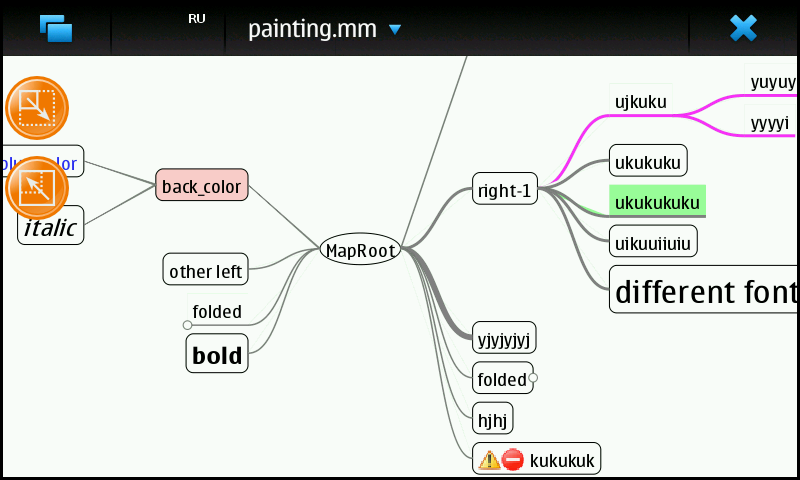
\includegraphics[width=1\linewidth]{main_view} 
% \caption{Отображение модели диаграммы связей}
% \label{ris:main_view}
% \end{figure}
% 
% \begin{figure}[h!] 
% \centering 
% 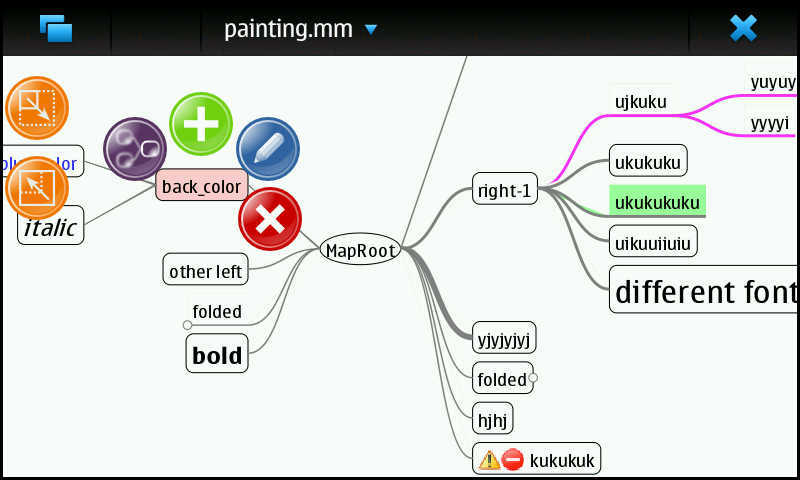
\includegraphics[width=0.6\linewidth]{context_menu} 
% \caption{Контекстное меню узла}
% \label{ris:context_menu}
% \end{figure}
% 
% \begin{figure}[h!]
% \begin{minipage}[h]{0.45\linewidth}
% \center{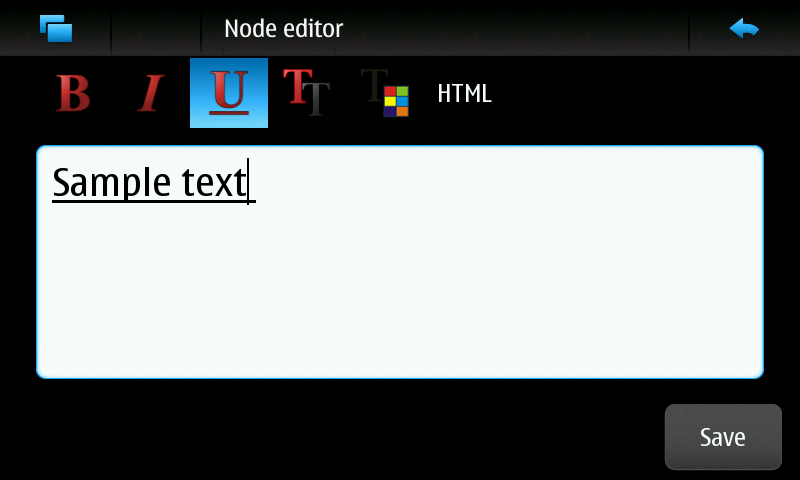
\includegraphics[width=1\linewidth]{text_dialog}} a) Главное окно редактора\\
% \end{minipage}
% \hfill
% \begin{minipage}[h]{0.45\linewidth}
% \center{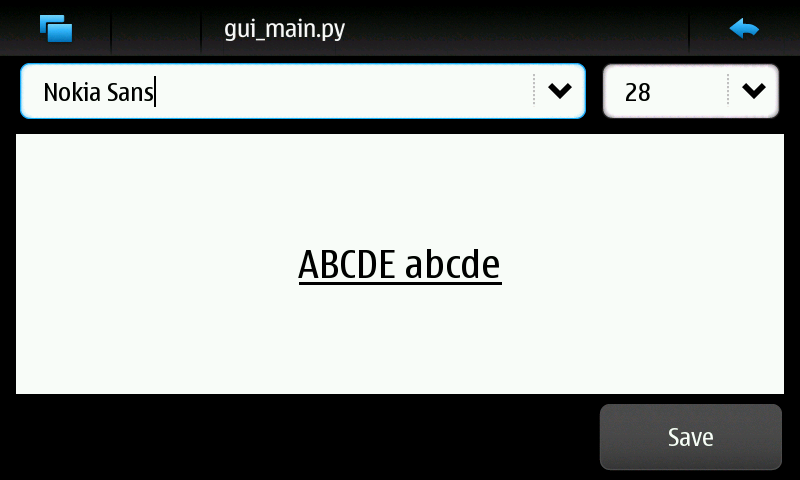
\includegraphics[width=1\linewidth]{font_dialog}} b) Диалог выбора шрифта\\
% \label{ris:font_dialog}
% \end{minipage}
% \vfill
% \begin{minipage}[h]{0.45\linewidth}
% \center{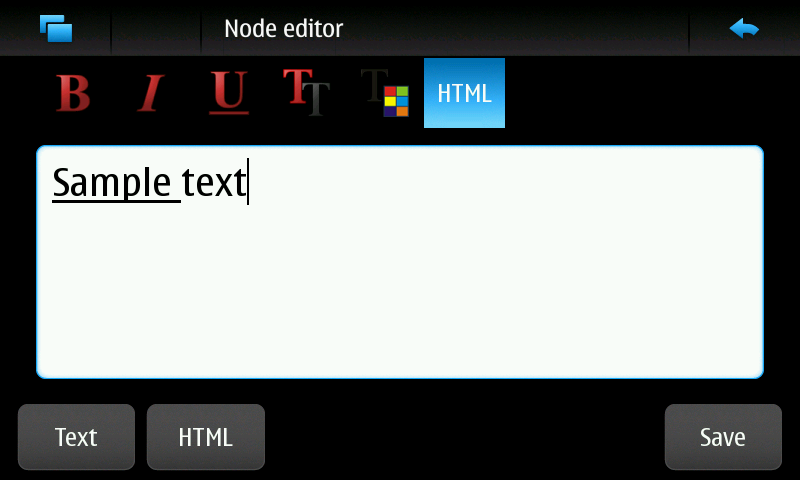
\includegraphics[width=1\linewidth]{html_editor}} c) Режим редактирования HTML\\
% \end{minipage}
% \hfill
% \begin{minipage}[h]{0.45\linewidth}
% \center{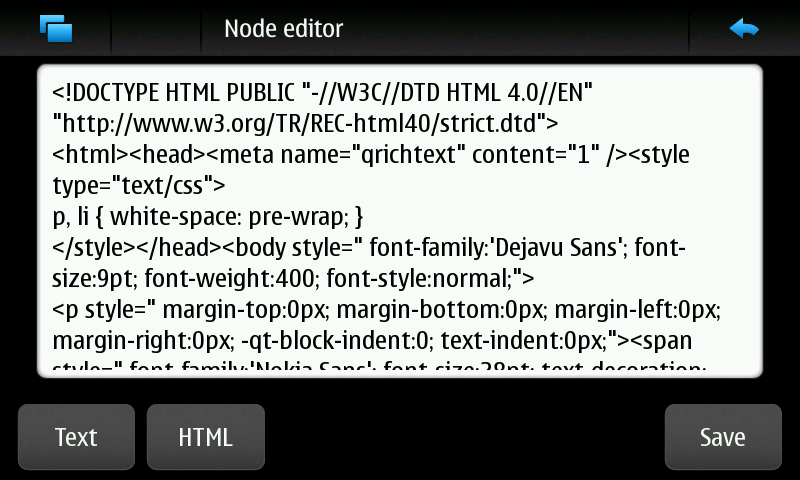
\includegraphics[width=1\linewidth]{html_source}} d) Редактирование исходного кода HTML\\
% \end{minipage}
% \caption{Редактор текста}
% \label{ris:text_editor}
% \end{figure}
% 
% \begin{figure}[h!] 
% \centering 
% 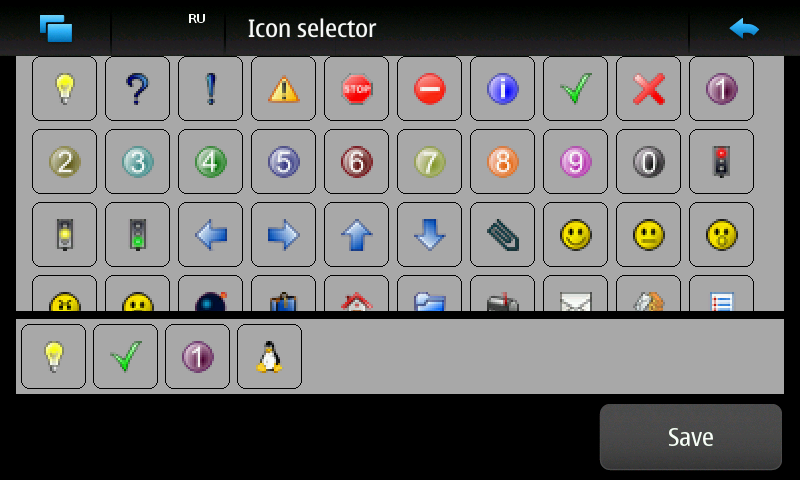
\includegraphics[width=1\linewidth]{icon_selector} 
% \caption{Диалог выбора иконок}
% \label{ris:icons_selector}
% \end{figure}
% \chapter{Диаграмма взаимодействия модели и вида}\label{ap:uml_scene}
% 
% \begin{figure}[h!] 
% \centering 
% 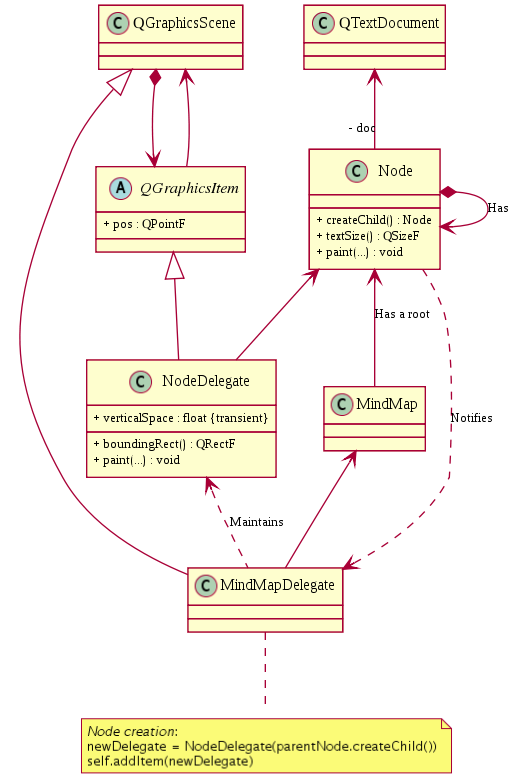
\includegraphics[width=0.5\linewidth]{uml_graphics} 
% \caption{Диаграмма взаимодействия модель-вид}
% \label{ris:uml_scene}
% \end{figure}
\newpage

\thispagestyle{empty}

\section*{Реферат}

\noindent
Отчёт 51 стр., 3 главы, 15 рис., 2 приложения, 10 источников литературы \\
\textbf{
РАЗРАБОТКА, СИСТЕМЫ УПРАВЛЕНИЯ ПРОЕКТАМИ, \\ REDMINE, RUBY ON RAILS,
ПЛАГИНЫ, ПАТЧИ, \\ ПОДДЕРЖКА РАСШИРЕНИЙ, OPEN SOURCE
}

Цель работы "--- разработать ряд расширений для системы управления проектами
Redmine.

В работе освещена разработка расширений для системы управления проектами
Redmine. Описаны детали реализации данных расширений. Усовершенствован процесс
подержки расширений с помощью инструмента Mercurial Queues. Приведены
результаты размещения разработанных расширений в открытом доступе.

Создано 6 расширений для Redmine. Внедрен усовершенствованный процесс поддержки
расширений. Получены отзывы и улучшения от сообщества разработчиков.

Разработанные расширения используются Ярославской лабораторией FRUCT.


%%% Local Variables: 
%%% mode: latex
%%% TeX-PDF-mode: t
%%% TeX-master: "diploma"
%%% End: 

\end{document}

%%% Local Variables: 
%%% mode: latex
%%% TeX-PDF-mode: t
%%% TeX-master: t
%%% End: 
